\documentclass[1p]{elsarticle_modified}
%\bibliographystyle{elsarticle-num}

%\usepackage[colorlinks]{hyperref}
%\usepackage{abbrmath_seonhwa} %\Abb, \Ascr, \Acal ,\Abf, \Afrak
\usepackage{amsfonts}
\usepackage{amssymb}
\usepackage{amsmath}
\usepackage{amsthm}
\usepackage{scalefnt}
\usepackage{amsbsy}
\usepackage{kotex}
\usepackage{caption}
\usepackage{subfig}
\usepackage{color}
\usepackage{graphicx}
\usepackage{xcolor} %% white, black, red, green, blue, cyan, magenta, yellow
\usepackage{float}
\usepackage{setspace}
\usepackage{hyperref}

\usepackage{tikz}
\usetikzlibrary{arrows}

\usepackage{multirow}
\usepackage{array} % fixed length table
\usepackage{hhline}

%%%%%%%%%%%%%%%%%%%%%
\makeatletter
\renewcommand*\env@matrix[1][\arraystretch]{%
	\edef\arraystretch{#1}%
	\hskip -\arraycolsep
	\let\@ifnextchar\new@ifnextchar
	\array{*\c@MaxMatrixCols c}}
\makeatother %https://tex.stackexchange.com/questions/14071/how-can-i-increase-the-line-spacing-in-a-matrix
%%%%%%%%%%%%%%%

\usepackage[normalem]{ulem}

\newcommand{\msout}[1]{\ifmmode\text{\sout{\ensuremath{#1}}}\else\sout{#1}\fi}
%SOURCE: \msout is \stkout macro in https://tex.stackexchange.com/questions/20609/strikeout-in-math-mode

\newcommand{\cancel}[1]{
	\ifmmode
	{\color{red}\msout{#1}}
	\else
	{\color{red}\sout{#1}}
	\fi
}

\newcommand{\add}[1]{
	{\color{blue}\uwave{#1}}
}

\newcommand{\replace}[2]{
	\ifmmode
	{\color{red}\msout{#1}}{\color{blue}\uwave{#2}}
	\else
	{\color{red}\sout{#1}}{\color{blue}\uwave{#2}}
	\fi
}

\newcommand{\Sol}{\mathcal{S}} %segment
\newcommand{\D}{D} %diagram
\newcommand{\A}{\mathcal{A}} %arc


%%%%%%%%%%%%%%%%%%%%%%%%%%%%%5 test

\def\sl{\operatorname{\textup{SL}}(2,\Cbb)}
\def\psl{\operatorname{\textup{PSL}}(2,\Cbb)}
\def\quan{\mkern 1mu \triangleright \mkern 1mu}

\theoremstyle{definition}
\newtheorem{thm}{Theorem}[section]
\newtheorem{prop}[thm]{Proposition}
\newtheorem{lem}[thm]{Lemma}
\newtheorem{ques}[thm]{Question}
\newtheorem{cor}[thm]{Corollary}
\newtheorem{defn}[thm]{Definition}
\newtheorem{exam}[thm]{Example}
\newtheorem{rmk}[thm]{Remark}
\newtheorem{alg}[thm]{Algorithm}

\newcommand{\I}{\sqrt{-1}}
\begin{document}

%\begin{frontmatter}
%
%\title{Boundary parabolic representations of knots up to 8 crossings}
%
%%% Group authors per affiliation:
%\author{Yunhi Cho} 
%\address{Department of Mathematics, University of Seoul, Seoul, Korea}
%\ead{yhcho@uos.ac.kr}
%
%
%\author{Seonhwa Kim} %\fnref{s_kim}}
%\address{Center for Geometry and Physics, Institute for Basic Science, Pohang, 37673, Korea}
%\ead{ryeona17@ibs.re.kr}
%
%\author{Hyuk Kim}
%\address{Department of Mathematical Sciences, Seoul National University, Seoul 08826, Korea}
%\ead{hyukkim@snu.ac.kr}
%
%\author{Seokbeom Yoon}
%\address{Department of Mathematical Sciences, Seoul National University, Seoul, 08826,  Korea}
%\ead{sbyoon15@snu.ac.kr}
%
%\begin{abstract}
%We find all boundary parabolic representation of knots up to 8 crossings.
%
%\end{abstract}
%\begin{keyword}
%    \MSC[2010] 57M25 
%\end{keyword}
%
%\end{frontmatter}

%\linenumbers
%\tableofcontents
%
\newcommand\colored[1]{\textcolor{white}{\rule[-0.35ex]{0.8em}{1.4ex}}\kern-0.8em\color{red} #1}%
%\newcommand\colored[1]{\textcolor{white}{ #1}\kern-2.17ex	\textcolor{white}{ #1}\kern-1.81ex	\textcolor{white}{ #1}\kern-2.15ex\color{red}#1	}

{\Large $\underline{12a_{0606}~(K12a_{0606})}$}

\setlength{\tabcolsep}{10pt}
\renewcommand{\arraystretch}{1.6}
\vspace{1cm}\begin{tabular}{m{100pt}>{\centering\arraybackslash}m{274pt}}
\multirow{5}{120pt}{
	\centering
	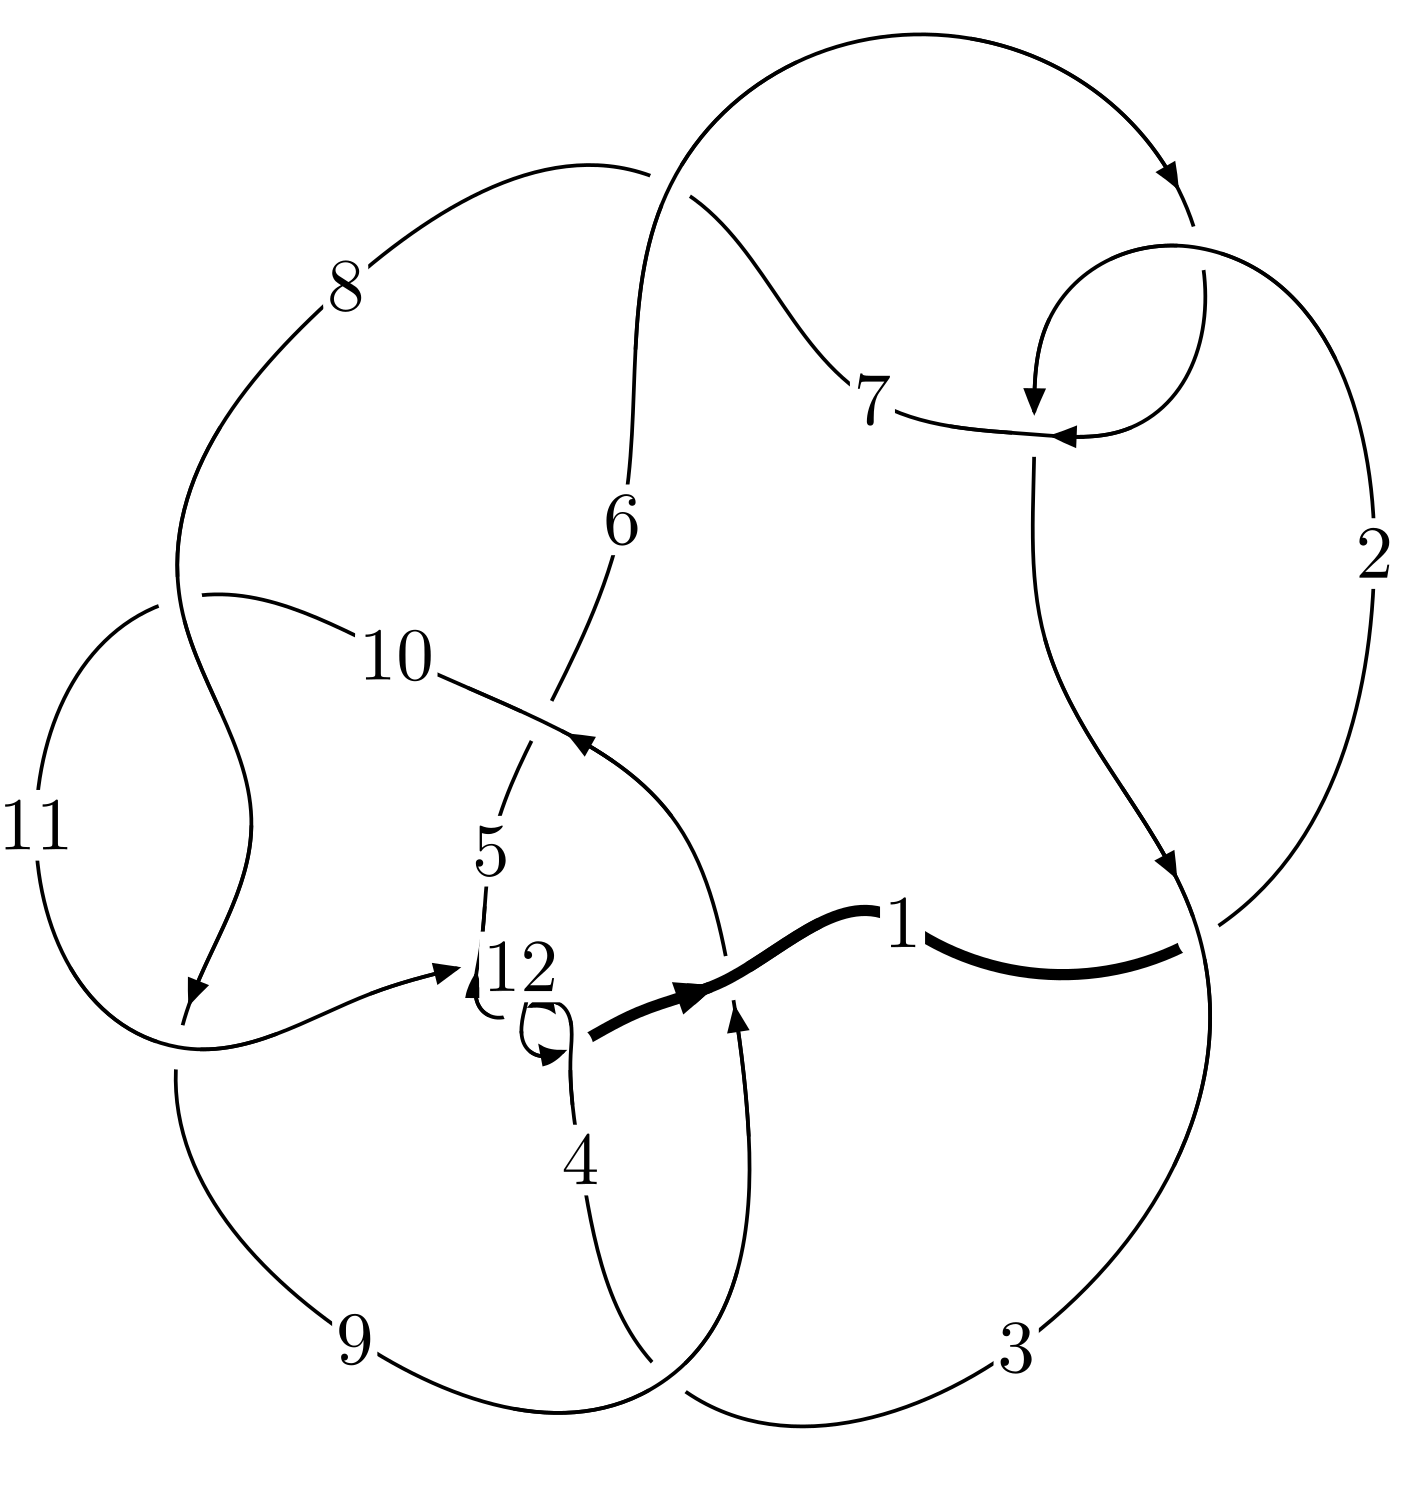
\includegraphics[width=112pt]{../../../GIT/diagram.site/Diagrams/png/1407_12a_0606.png}\\
\ \ \ A knot diagram\footnotemark}&
\allowdisplaybreaks
\textbf{Linearized knot diagam} \\
\cline{2-2}
 &
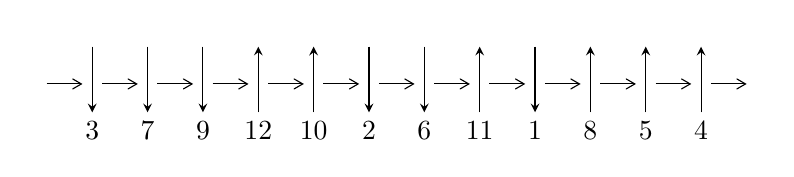
\begin{tikzpicture}[x=20pt, y=17pt]
	% nodes
	\node (C0) at (0, 0) {};
	\node (C1) at (1, 0) {};
	\node (C1U) at (1, +1) {};
	\node (C1D) at (1, -1) {3};

	\node (C2) at (2, 0) {};
	\node (C2U) at (2, +1) {};
	\node (C2D) at (2, -1) {7};

	\node (C3) at (3, 0) {};
	\node (C3U) at (3, +1) {};
	\node (C3D) at (3, -1) {9};

	\node (C4) at (4, 0) {};
	\node (C4U) at (4, +1) {};
	\node (C4D) at (4, -1) {12};

	\node (C5) at (5, 0) {};
	\node (C5U) at (5, +1) {};
	\node (C5D) at (5, -1) {10};

	\node (C6) at (6, 0) {};
	\node (C6U) at (6, +1) {};
	\node (C6D) at (6, -1) {2};

	\node (C7) at (7, 0) {};
	\node (C7U) at (7, +1) {};
	\node (C7D) at (7, -1) {6};

	\node (C8) at (8, 0) {};
	\node (C8U) at (8, +1) {};
	\node (C8D) at (8, -1) {11};

	\node (C9) at (9, 0) {};
	\node (C9U) at (9, +1) {};
	\node (C9D) at (9, -1) {1};

	\node (C10) at (10, 0) {};
	\node (C10U) at (10, +1) {};
	\node (C10D) at (10, -1) {8};

	\node (C11) at (11, 0) {};
	\node (C11U) at (11, +1) {};
	\node (C11D) at (11, -1) {5};

	\node (C12) at (12, 0) {};
	\node (C12U) at (12, +1) {};
	\node (C12D) at (12, -1) {4};
	\node (C13) at (13, 0) {};

	% arrows
	\draw[->,>={angle 60}]
	(C0) edge (C1) (C1) edge (C2) (C2) edge (C3) (C3) edge (C4) (C4) edge (C5) (C5) edge (C6) (C6) edge (C7) (C7) edge (C8) (C8) edge (C9) (C9) edge (C10) (C10) edge (C11) (C11) edge (C12) (C12) edge (C13) ;	\draw[->,>=stealth]
	(C1U) edge (C1D) (C2U) edge (C2D) (C3U) edge (C3D) (C4D) edge (C4U) (C5D) edge (C5U) (C6U) edge (C6D) (C7U) edge (C7D) (C8D) edge (C8U) (C9U) edge (C9D) (C10D) edge (C10U) (C11D) edge (C11U) (C12D) edge (C12U) ;
	\end{tikzpicture} \\
\hhline{~~} \\& 
\textbf{Solving Sequence} \\ \cline{2-2} 
 &
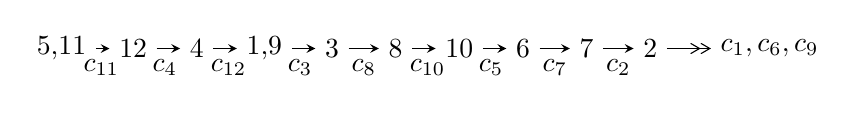
\begin{tikzpicture}[x=23pt, y=7pt]
	% node
	\node (A0) at (-1/8, 0) {5,11};
	\node (A1) at (1, 0) {12};
	\node (A2) at (2, 0) {4};
	\node (A3) at (49/16, 0) {1,9};
	\node (A4) at (33/8, 0) {3};
	\node (A5) at (41/8, 0) {8};
	\node (A6) at (49/8, 0) {10};
	\node (A7) at (57/8, 0) {6};
	\node (A8) at (65/8, 0) {7};
	\node (A9) at (73/8, 0) {2};
	\node (C1) at (1/2, -1) {$c_{11}$};
	\node (C2) at (3/2, -1) {$c_{4}$};
	\node (C3) at (5/2, -1) {$c_{12}$};
	\node (C4) at (29/8, -1) {$c_{3}$};
	\node (C5) at (37/8, -1) {$c_{8}$};
	\node (C6) at (45/8, -1) {$c_{10}$};
	\node (C7) at (53/8, -1) {$c_{5}$};
	\node (C8) at (61/8, -1) {$c_{7}$};
	\node (C9) at (69/8, -1) {$c_{2}$};
	\node (A10) at (11, 0) {$c_{1},c_{6},c_{9}$};

	% edge
	\draw[->,>=stealth]	
	(A0) edge (A1) (A1) edge (A2) (A2) edge (A3) (A3) edge (A4) (A4) edge (A5) (A5) edge (A6) (A6) edge (A7) (A7) edge (A8) (A8) edge (A9) ;
	\draw[->>,>={angle 60}]	
	(A9) edge (A10);
\end{tikzpicture} \\ 

\end{tabular} \\

\footnotetext{
The image of knot diagram is generated by the software ``\textbf{Draw programme}" developed by Andrew Bartholomew(\url{http://www.layer8.co.uk/maths/draw/index.htm\#Running-draw}), where we modified some parts for our purpose(\url{https://github.com/CATsTAILs/LinksPainter}).
}\phantom \\ \newline 
\centering \textbf{Ideals for irreducible components\footnotemark of $X_{\text{par}}$} 
 
\begin{align*}
I^u_{1}&=\langle 
-6.74463\times10^{127} u^{83}+1.59218\times10^{128} u^{82}+\cdots+3.44840\times10^{128} b-2.29894\times10^{128},\\
\phantom{I^u_{1}}&\phantom{= \langle  }-3.01103\times10^{128} u^{83}+9.56492\times10^{128} u^{82}+\cdots+3.44840\times10^{128} a+2.95385\times10^{128},\\
\phantom{I^u_{1}}&\phantom{= \langle  }u^{84}-3 u^{83}+\cdots-2 u+1\rangle \\
\\
\end{align*}
\raggedright * 1 irreducible components of $\dim_{\mathbb{C}}=0$, with total 84 representations.\\
\footnotetext{All coefficients of polynomials are rational numbers. But the coefficients are sometimes approximated in decimal forms when there is not enough margin.}
\newpage
\renewcommand{\arraystretch}{1}
\centering \section*{I. $I^u_{1}= \langle -6.74\times10^{127} u^{83}+1.59\times10^{128} u^{82}+\cdots+3.45\times10^{128} b-2.30\times10^{128},\;-3.01\times10^{128} u^{83}+9.56\times10^{128} u^{82}+\cdots+3.45\times10^{128} a+2.95\times10^{128},\;u^{84}-3 u^{83}+\cdots-2 u+1 \rangle$}
\flushleft \textbf{(i) Arc colorings}\\
\begin{tabular}{m{7pt} m{180pt} m{7pt} m{180pt} }
\flushright $a_{5}=$&$\begin{pmatrix}0\\u\end{pmatrix}$ \\
\flushright $a_{11}=$&$\begin{pmatrix}1\\0\end{pmatrix}$ \\
\flushright $a_{12}=$&$\begin{pmatrix}1\\- u^2\end{pmatrix}$ \\
\flushright $a_{4}=$&$\begin{pmatrix}- u\\u^3+u\end{pmatrix}$ \\
\flushright $a_{1}=$&$\begin{pmatrix}u^2+1\\- u^4-2 u^2\end{pmatrix}$ \\
\flushright $a_{9}=$&$\begin{pmatrix}0.873168 u^{83}-2.77373 u^{82}+\cdots-12.8263 u-0.856587\\0.195587 u^{83}-0.461715 u^{82}+\cdots+0.0665166 u+0.666670\end{pmatrix}$ \\
\flushright $a_{3}=$&$\begin{pmatrix}-3.59196 u^{83}+30.5345 u^{82}+\cdots-21.0237 u+15.6011\\1.26933 u^{83}-3.73690 u^{82}+\cdots+3.06667 u-1.23274\end{pmatrix}$ \\
\flushright $a_{8}=$&$\begin{pmatrix}0.677581 u^{83}-2.31201 u^{82}+\cdots-12.8928 u-1.52326\\0.195587 u^{83}-0.461715 u^{82}+\cdots+0.0665166 u+0.666670\end{pmatrix}$ \\
\flushright $a_{10}=$&$\begin{pmatrix}0.681360 u^{83}-2.29472 u^{82}+\cdots-12.9913 u-0.464526\\0.284715 u^{83}-0.696196 u^{82}+\cdots+0.0869901 u+0.486513\end{pmatrix}$ \\
\flushright $a_{6}=$&$\begin{pmatrix}4.98831 u^{83}-35.4998 u^{82}+\cdots+29.5605 u-5.16163\\-0.534425 u^{83}+1.36777 u^{82}+\cdots+1.91603 u-0.186017\end{pmatrix}$ \\
\flushright $a_{7}=$&$\begin{pmatrix}-20.3353 u^{83}+57.5455 u^{82}+\cdots-13.6819 u-4.17574\\0.951845 u^{83}-1.18145 u^{82}+\cdots-1.05176 u-0.348775\end{pmatrix}$ \\
\flushright $a_{2}=$&$\begin{pmatrix}-19.4294 u^{83}+55.1803 u^{82}+\cdots-13.4541 u+2.38119\\0.336489 u^{83}+0.297026 u^{82}+\cdots-1.10082 u+0.813010\end{pmatrix}$\\&\end{tabular}
\flushleft \textbf{(ii) Obstruction class $= -1$}\\~\\
\flushleft \textbf{(iii) Cusp Shapes $= -3.96005 u^{83}+5.91536 u^{82}+\cdots+26.5735 u-14.4137$}\\~\\
\newpage\renewcommand{\arraystretch}{1}
\flushleft \textbf{(iv) u-Polynomials at the component}\newline \\
\begin{tabular}{m{50pt}|m{274pt}}
Crossings & \hspace{64pt}u-Polynomials at each crossing \\
\hline $$\begin{aligned}c_{1},c_{7}\end{aligned}$$&$\begin{aligned}
&u^{84}+23 u^{83}+\cdots+6 u+1
\end{aligned}$\\
\hline $$\begin{aligned}c_{2},c_{6}\end{aligned}$$&$\begin{aligned}
&u^{84}- u^{83}+\cdots-3 u^2+1
\end{aligned}$\\
\hline $$\begin{aligned}c_{3}\end{aligned}$$&$\begin{aligned}
&u^{84}-65 u^{83}+\cdots+2 u+1
\end{aligned}$\\
\hline $$\begin{aligned}c_{4},c_{11},c_{12}\end{aligned}$$&$\begin{aligned}
&u^{84}+3 u^{83}+\cdots+2 u+1
\end{aligned}$\\
\hline $$\begin{aligned}c_{5}\end{aligned}$$&$\begin{aligned}
&u^{84}+63 u^{83}+\cdots+57180 u-86897
\end{aligned}$\\
\hline $$\begin{aligned}c_{8},c_{10}\end{aligned}$$&$\begin{aligned}
&u^{84}+u^{83}+\cdots-34 u+1
\end{aligned}$\\
\hline $$\begin{aligned}c_{9}\end{aligned}$$&$\begin{aligned}
&u^{84}+7 u^{83}+\cdots+8 u+1
\end{aligned}$\\
\hline
\end{tabular}\\~\\
\newpage\renewcommand{\arraystretch}{1}
\flushleft \textbf{(v) Riley Polynomials at the component}\newline \\
\begin{tabular}{m{50pt}|m{274pt}}
Crossings & \hspace{64pt}Riley Polynomials at each crossing \\
\hline $$\begin{aligned}c_{1},c_{7}\end{aligned}$$&$\begin{aligned}
&y^{84}+77 y^{83}+\cdots-6 y+1
\end{aligned}$\\
\hline $$\begin{aligned}c_{2},c_{6}\end{aligned}$$&$\begin{aligned}
&y^{84}-23 y^{83}+\cdots-6 y+1
\end{aligned}$\\
\hline $$\begin{aligned}c_{3}\end{aligned}$$&$\begin{aligned}
&y^{84}-1667 y^{83}+\cdots+622 y+1
\end{aligned}$\\
\hline $$\begin{aligned}c_{4},c_{11},c_{12}\end{aligned}$$&$\begin{aligned}
&y^{84}+81 y^{83}+\cdots-6 y+1
\end{aligned}$\\
\hline $$\begin{aligned}c_{5}\end{aligned}$$&$\begin{aligned}
&y^{84}-1711 y^{83}+\cdots-279584806794 y+7551088609
\end{aligned}$\\
\hline $$\begin{aligned}c_{8},c_{10}\end{aligned}$$&$\begin{aligned}
&y^{84}-55 y^{83}+\cdots+754 y+1
\end{aligned}$\\
\hline $$\begin{aligned}c_{9}\end{aligned}$$&$\begin{aligned}
&y^{84}-3 y^{83}+\cdots+226 y+1
\end{aligned}$\\
\hline
\end{tabular}\\~\\
\newpage\flushleft \textbf{(vi) Complex Volumes and Cusp Shapes}
$$\begin{array}{c|c|c}  
\text{Solutions to }I^u_{1}& \I (\text{vol} + \sqrt{-1}CS) & \text{Cusp shape}\\
 \hline 
\begin{aligned}
u &= -0.841085 + 0.491787 I \\
a &= \phantom{-}0.458081 + 0.952887 I \\
b &= -1.36898 + 0.43042 I\end{aligned}
 & \phantom{-}8.55629 - 6.70046 I & \phantom{-0.000000 } 0 \\ \hline\begin{aligned}
u &= -0.841085 - 0.491787 I \\
a &= \phantom{-}0.458081 - 0.952887 I \\
b &= -1.36898 - 0.43042 I\end{aligned}
 & \phantom{-}8.55629 + 6.70046 I & \phantom{-0.000000 } 0 \\ \hline\begin{aligned}
u &= \phantom{-}0.395039 + 0.889142 I \\
a &= \phantom{-}0.299173 - 0.145406 I \\
b &= -0.578416 + 0.157326 I\end{aligned}
 & -1.33288 - 2.11542 I & \phantom{-0.000000 } 0 \\ \hline\begin{aligned}
u &= \phantom{-}0.395039 - 0.889142 I \\
a &= \phantom{-}0.299173 + 0.145406 I \\
b &= -0.578416 - 0.157326 I\end{aligned}
 & -1.33288 + 2.11542 I & \phantom{-0.000000 } 0 \\ \hline\begin{aligned}
u &= \phantom{-}0.830958 + 0.488150 I \\
a &= \phantom{-}0.499768 - 0.996423 I \\
b &= -1.36888 - 0.48638 I\end{aligned}
 & \phantom{-}7.7472 + 13.0248 I & \phantom{-0.000000 } 0 \\ \hline\begin{aligned}
u &= \phantom{-}0.830958 - 0.488150 I \\
a &= \phantom{-}0.499768 + 0.996423 I \\
b &= -1.36888 + 0.48638 I\end{aligned}
 & \phantom{-}7.7472 - 13.0248 I & \phantom{-0.000000 } 0 \\ \hline\begin{aligned}
u &= \phantom{-}0.857305 + 0.428649 I \\
a &= \phantom{-}0.649452 - 0.755906 I \\
b &= -1.126900 - 0.419335 I\end{aligned}
 & \phantom{-}0.10242 + 7.46364 I & \phantom{-0.000000 } 0 \\ \hline\begin{aligned}
u &= \phantom{-}0.857305 - 0.428649 I \\
a &= \phantom{-}0.649452 + 0.755906 I \\
b &= -1.126900 + 0.419335 I\end{aligned}
 & \phantom{-}0.10242 - 7.46364 I & \phantom{-0.000000 } 0 \\ \hline\begin{aligned}
u &= \phantom{-}0.808233 + 0.660887 I \\
a &= -0.087128 - 0.445454 I \\
b &= -1.260470 + 0.320226 I\end{aligned}
 & \phantom{-}7.27039 - 7.59198 I & \phantom{-0.000000 } 0 \\ \hline\begin{aligned}
u &= \phantom{-}0.808233 - 0.660887 I \\
a &= -0.087128 + 0.445454 I \\
b &= -1.260470 - 0.320226 I\end{aligned}
 & \phantom{-}7.27039 + 7.59198 I & \phantom{-0.000000 } 0\\
 \hline 
 \end{array}$$\newpage$$\begin{array}{c|c|c}  
\text{Solutions to }I^u_{1}& \I (\text{vol} + \sqrt{-1}CS) & \text{Cusp shape}\\
 \hline 
\begin{aligned}
u &= -0.951611 + 0.456794 I \\
a &= \phantom{-}0.460493 + 0.572983 I \\
b &= -1.131900 + 0.209269 I\end{aligned}
 & \phantom{-}3.49418 - 3.27329 I & \phantom{-0.000000 } 0 \\ \hline\begin{aligned}
u &= -0.951611 - 0.456794 I \\
a &= \phantom{-}0.460493 - 0.572983 I \\
b &= -1.131900 - 0.209269 I\end{aligned}
 & \phantom{-}3.49418 + 3.27329 I & \phantom{-0.000000 } 0 \\ \hline\begin{aligned}
u &= -0.836469 + 0.662101 I \\
a &= -0.033924 + 0.476709 I \\
b &= -1.262520 - 0.240610 I\end{aligned}
 & \phantom{-}8.09488 + 1.17071 I & \phantom{-0.000000 } 0 \\ \hline\begin{aligned}
u &= -0.836469 - 0.662101 I \\
a &= -0.033924 - 0.476709 I \\
b &= -1.262520 + 0.240610 I\end{aligned}
 & \phantom{-}8.09488 - 1.17071 I & \phantom{-0.000000 } 0 \\ \hline\begin{aligned}
u &= \phantom{-}0.925944\phantom{ +0.000000I} \\
a &= \phantom{-}0.813290\phantom{ +0.000000I} \\
b &= -0.772047\phantom{ +0.000000I}\end{aligned}
 & -1.56515\phantom{ +0.000000I} & \phantom{-0.000000 } 0 \\ \hline\begin{aligned}
u &= \phantom{-}0.007440 + 1.230010 I \\
a &= \phantom{-}1.56019 + 0.08942 I \\
b &= \phantom{-}1.83888 + 0.03682 I\end{aligned}
 & \phantom{-}4.48868 + 3.01865 I & \phantom{-0.000000 } 0 \\ \hline\begin{aligned}
u &= \phantom{-}0.007440 - 1.230010 I \\
a &= \phantom{-}1.56019 - 0.08942 I \\
b &= \phantom{-}1.83888 - 0.03682 I\end{aligned}
 & \phantom{-}4.48868 - 3.01865 I & \phantom{-0.000000 } 0 \\ \hline\begin{aligned}
u &= \phantom{-}0.511792 + 1.130900 I \\
a &= \phantom{-}0.244866 - 0.380174 I \\
b &= -0.757105 - 0.005600 I\end{aligned}
 & -1.34459 - 2.08242 I & \phantom{-0.000000 } 0 \\ \hline\begin{aligned}
u &= \phantom{-}0.511792 - 1.130900 I \\
a &= \phantom{-}0.244866 + 0.380174 I \\
b &= -0.757105 + 0.005600 I\end{aligned}
 & -1.34459 + 2.08242 I & \phantom{-0.000000 } 0 \\ \hline\begin{aligned}
u &= \phantom{-}0.036951 + 1.305380 I \\
a &= \phantom{-}0.565454 + 0.681799 I \\
b &= \phantom{-}1.43082 + 0.21052 I\end{aligned}
 & -1.38495 + 1.38895 I & \phantom{-0.000000 } 0\\
 \hline 
 \end{array}$$\newpage$$\begin{array}{c|c|c}  
\text{Solutions to }I^u_{1}& \I (\text{vol} + \sqrt{-1}CS) & \text{Cusp shape}\\
 \hline 
\begin{aligned}
u &= \phantom{-}0.036951 - 1.305380 I \\
a &= \phantom{-}0.565454 - 0.681799 I \\
b &= \phantom{-}1.43082 - 0.21052 I\end{aligned}
 & -1.38495 - 1.38895 I & \phantom{-0.000000 } 0 \\ \hline\begin{aligned}
u &= \phantom{-}0.488142 + 0.482785 I \\
a &= \phantom{-}0.031188 + 0.410920 I \\
b &= -0.148976 + 0.767569 I\end{aligned}
 & -2.79385 + 3.17067 I & -6.19468 - 7.29951 I \\ \hline\begin{aligned}
u &= \phantom{-}0.488142 - 0.482785 I \\
a &= \phantom{-}0.031188 - 0.410920 I \\
b &= -0.148976 - 0.767569 I\end{aligned}
 & -2.79385 - 3.17067 I & -6.19468 + 7.29951 I \\ \hline\begin{aligned}
u &= \phantom{-}0.142621 + 1.317630 I \\
a &= \phantom{-}1.00564 + 1.87617 I \\
b &= \phantom{-}1.38650 + 0.96883 I\end{aligned}
 & \phantom{-}2.97262 + 1.36691 I & \phantom{-0.000000 } 0 \\ \hline\begin{aligned}
u &= \phantom{-}0.142621 - 1.317630 I \\
a &= \phantom{-}1.00564 - 1.87617 I \\
b &= \phantom{-}1.38650 - 0.96883 I\end{aligned}
 & \phantom{-}2.97262 - 1.36691 I & \phantom{-0.000000 } 0 \\ \hline\begin{aligned}
u &= \phantom{-}0.544314 + 0.397133 I \\
a &= -0.143255 + 0.627268 I \\
b &= \phantom{-}0.132496 + 1.098020 I\end{aligned}
 & \phantom{-}3.07508 + 7.54785 I & \phantom{-}1.67086 - 9.24892 I \\ \hline\begin{aligned}
u &= \phantom{-}0.544314 - 0.397133 I \\
a &= -0.143255 - 0.627268 I \\
b &= \phantom{-}0.132496 - 1.098020 I\end{aligned}
 & \phantom{-}3.07508 - 7.54785 I & \phantom{-}1.67086 + 9.24892 I \\ \hline\begin{aligned}
u &= -0.149362 + 1.325160 I \\
a &= \phantom{-}0.94788 - 1.95347 I \\
b &= \phantom{-}1.32824 - 1.03783 I\end{aligned}
 & \phantom{-}2.73190 - 7.38832 I & \phantom{-0.000000 } 0 \\ \hline\begin{aligned}
u &= -0.149362 - 1.325160 I \\
a &= \phantom{-}0.94788 + 1.95347 I \\
b &= \phantom{-}1.32824 + 1.03783 I\end{aligned}
 & \phantom{-}2.73190 + 7.38832 I & \phantom{-0.000000 } 0 \\ \hline\begin{aligned}
u &= \phantom{-}0.083022 + 1.342940 I \\
a &= \phantom{-}0.56214 + 1.54984 I \\
b &= \phantom{-}1.170010 + 0.494704 I\end{aligned}
 & -2.00569 + 1.65992 I & \phantom{-0.000000 } 0\\
 \hline 
 \end{array}$$\newpage$$\begin{array}{c|c|c}  
\text{Solutions to }I^u_{1}& \I (\text{vol} + \sqrt{-1}CS) & \text{Cusp shape}\\
 \hline 
\begin{aligned}
u &= \phantom{-}0.083022 - 1.342940 I \\
a &= \phantom{-}0.56214 - 1.54984 I \\
b &= \phantom{-}1.170010 - 0.494704 I\end{aligned}
 & -2.00569 - 1.65992 I & \phantom{-0.000000 } 0 \\ \hline\begin{aligned}
u &= -0.530735 + 0.378249 I \\
a &= -0.112600 - 0.681713 I \\
b &= \phantom{-}0.237830 - 1.043500 I\end{aligned}
 & \phantom{-}3.56923 - 1.66317 I & \phantom{-}2.96826 + 4.34619 I \\ \hline\begin{aligned}
u &= -0.530735 - 0.378249 I \\
a &= -0.112600 + 0.681713 I \\
b &= \phantom{-}0.237830 + 1.043500 I\end{aligned}
 & \phantom{-}3.56923 + 1.66317 I & \phantom{-}2.96826 - 4.34619 I \\ \hline\begin{aligned}
u &= -0.124292 + 1.367670 I \\
a &= \phantom{-}0.62258 - 1.80283 I \\
b &= \phantom{-}0.932347 - 0.818895 I\end{aligned}
 & -3.57253 - 4.34184 I & \phantom{-0.000000 } 0 \\ \hline\begin{aligned}
u &= -0.124292 - 1.367670 I \\
a &= \phantom{-}0.62258 + 1.80283 I \\
b &= \phantom{-}0.932347 + 0.818895 I\end{aligned}
 & -3.57253 + 4.34184 I & \phantom{-0.000000 } 0 \\ \hline\begin{aligned}
u &= -0.058832 + 1.393540 I \\
a &= \phantom{-}0.66333 - 2.39711 I \\
b &= \phantom{-}0.870044 - 0.206745 I\end{aligned}
 & -4.73549 - 0.52192 I & \phantom{-0.000000 } 0 \\ \hline\begin{aligned}
u &= -0.058832 - 1.393540 I \\
a &= \phantom{-}0.66333 + 2.39711 I \\
b &= \phantom{-}0.870044 + 0.206745 I\end{aligned}
 & -4.73549 + 0.52192 I & \phantom{-0.000000 } 0 \\ \hline\begin{aligned}
u &= -0.007361 + 1.411650 I \\
a &= -5.3069 - 21.3383 I \\
b &= \phantom{-}0.997042 - 0.002480 I\end{aligned}
 & -0.27149 + 2.82297 I & \phantom{-0.000000 } 0 \\ \hline\begin{aligned}
u &= -0.007361 - 1.411650 I \\
a &= -5.3069 + 21.3383 I \\
b &= \phantom{-}0.997042 + 0.002480 I\end{aligned}
 & -0.27149 - 2.82297 I & \phantom{-0.000000 } 0 \\ \hline\begin{aligned}
u &= -0.02514 + 1.42770 I \\
a &= \phantom{-}0.943312 - 0.184770 I \\
b &= \phantom{-}0.0166012 - 0.0228494 I\end{aligned}
 & -1.89129 - 2.85052 I & \phantom{-0.000000 } 0\\
 \hline 
 \end{array}$$\newpage$$\begin{array}{c|c|c}  
\text{Solutions to }I^u_{1}& \I (\text{vol} + \sqrt{-1}CS) & \text{Cusp shape}\\
 \hline 
\begin{aligned}
u &= -0.02514 - 1.42770 I \\
a &= \phantom{-}0.943312 + 0.184770 I \\
b &= \phantom{-}0.0166012 + 0.0228494 I\end{aligned}
 & -1.89129 + 2.85052 I & \phantom{-0.000000 } 0 \\ \hline\begin{aligned}
u &= \phantom{-}0.450025 + 0.338178 I \\
a &= \phantom{-}1.89922 + 0.06419 I \\
b &= \phantom{-}0.156737 - 0.547212 I\end{aligned}
 & \phantom{-}3.05606 - 4.29554 I & \phantom{-}1.23916 + 0.97121 I \\ \hline\begin{aligned}
u &= \phantom{-}0.450025 - 0.338178 I \\
a &= \phantom{-}1.89922 - 0.06419 I \\
b &= \phantom{-}0.156737 + 0.547212 I\end{aligned}
 & \phantom{-}3.05606 + 4.29554 I & \phantom{-}1.23916 - 0.97121 I \\ \hline\begin{aligned}
u &= -0.532578 + 0.127338 I \\
a &= -0.482244 - 0.702775 I \\
b &= \phantom{-}1.45794 - 0.58858 I\end{aligned}
 & \phantom{-}7.22969 - 4.94035 I & \phantom{-}8.76064 + 6.43722 I \\ \hline\begin{aligned}
u &= -0.532578 - 0.127338 I \\
a &= -0.482244 + 0.702775 I \\
b &= \phantom{-}1.45794 + 0.58858 I\end{aligned}
 & \phantom{-}7.22969 + 4.94035 I & \phantom{-}8.76064 - 6.43722 I \\ \hline\begin{aligned}
u &= \phantom{-}0.530525 + 0.109986 I \\
a &= -0.527197 + 0.634287 I \\
b &= \phantom{-}1.50206 + 0.51079 I\end{aligned}
 & \phantom{-}7.37206 - 1.04586 I & \phantom{-}9.31067 - 0.66517 I \\ \hline\begin{aligned}
u &= \phantom{-}0.530525 - 0.109986 I \\
a &= -0.527197 - 0.634287 I \\
b &= \phantom{-}1.50206 - 0.51079 I\end{aligned}
 & \phantom{-}7.37206 + 1.04586 I & \phantom{-}9.31067 + 0.66517 I \\ \hline\begin{aligned}
u &= -0.18758 + 1.44911 I \\
a &= -0.32881 - 1.77671 I \\
b &= -0.020646 - 1.346400 I\end{aligned}
 & -2.33863 - 4.29175 I & \phantom{-0.000000 } 0 \\ \hline\begin{aligned}
u &= -0.18758 - 1.44911 I \\
a &= -0.32881 + 1.77671 I \\
b &= -0.020646 + 1.346400 I\end{aligned}
 & -2.33863 + 4.29175 I & \phantom{-0.000000 } 0 \\ \hline\begin{aligned}
u &= \phantom{-}0.537541\phantom{ +0.000000I} \\
a &= \phantom{-}1.24481\phantom{ +0.000000I} \\
b &= -0.258009\phantom{ +0.000000I}\end{aligned}
 & -1.72341\phantom{ +0.000000I} & -5.57880\phantom{ +0.000000I}\\
 \hline 
 \end{array}$$\newpage$$\begin{array}{c|c|c}  
\text{Solutions to }I^u_{1}& \I (\text{vol} + \sqrt{-1}CS) & \text{Cusp shape}\\
 \hline 
\begin{aligned}
u &= -0.407510 + 0.345674 I \\
a &= \phantom{-}1.99195 - 0.30079 I \\
b &= \phantom{-}0.300889 + 0.482319 I\end{aligned}
 & \phantom{-}3.44624 - 1.42162 I & \phantom{-}2.41052 + 4.86035 I \\ \hline\begin{aligned}
u &= -0.407510 - 0.345674 I \\
a &= \phantom{-}1.99195 + 0.30079 I \\
b &= \phantom{-}0.300889 - 0.482319 I\end{aligned}
 & \phantom{-}3.44624 + 1.42162 I & \phantom{-}2.41052 - 4.86035 I \\ \hline\begin{aligned}
u &= \phantom{-}0.19354 + 1.45472 I \\
a &= -0.43885 + 1.77233 I \\
b &= -0.106526 + 1.390560 I\end{aligned}
 & -2.91247 + 10.25220 I & \phantom{-0.000000 } 0 \\ \hline\begin{aligned}
u &= \phantom{-}0.19354 - 1.45472 I \\
a &= -0.43885 - 1.77233 I \\
b &= -0.106526 - 1.390560 I\end{aligned}
 & -2.91247 - 10.25220 I & \phantom{-0.000000 } 0 \\ \hline\begin{aligned}
u &= -0.349251 + 0.398009 I \\
a &= \phantom{-}0.463559 - 0.576542 I \\
b &= \phantom{-}0.121636 - 0.363687 I\end{aligned}
 & \phantom{-}0.097200 - 1.073830 I & \phantom{-}1.41884 + 6.13630 I \\ \hline\begin{aligned}
u &= -0.349251 - 0.398009 I \\
a &= \phantom{-}0.463559 + 0.576542 I \\
b &= \phantom{-}0.121636 + 0.363687 I\end{aligned}
 & \phantom{-}0.097200 + 1.073830 I & \phantom{-}1.41884 - 6.13630 I \\ \hline\begin{aligned}
u &= -0.14497 + 1.47396 I \\
a &= -0.115149 - 1.228520 I \\
b &= -0.119724 - 0.853117 I\end{aligned}
 & -6.10460 - 2.97941 I & \phantom{-0.000000 } 0 \\ \hline\begin{aligned}
u &= -0.14497 - 1.47396 I \\
a &= -0.115149 + 1.228520 I \\
b &= -0.119724 + 0.853117 I\end{aligned}
 & -6.10460 + 2.97941 I & \phantom{-0.000000 } 0 \\ \hline\begin{aligned}
u &= \phantom{-}0.17702 + 1.48022 I \\
a &= -0.45899 + 1.37729 I \\
b &= -0.290897 + 1.109090 I\end{aligned}
 & -9.16614 + 5.65167 I & \phantom{-0.000000 } 0 \\ \hline\begin{aligned}
u &= \phantom{-}0.17702 - 1.48022 I \\
a &= -0.45899 - 1.37729 I \\
b &= -0.290897 - 1.109090 I\end{aligned}
 & -9.16614 - 5.65167 I & \phantom{-0.000000 } 0\\
 \hline 
 \end{array}$$\newpage$$\begin{array}{c|c|c}  
\text{Solutions to }I^u_{1}& \I (\text{vol} + \sqrt{-1}CS) & \text{Cusp shape}\\
 \hline 
\begin{aligned}
u &= \phantom{-}0.33509 + 1.46619 I \\
a &= \phantom{-}0.026808 - 1.216630 I \\
b &= -1.038500 - 0.483600 I\end{aligned}
 & -6.87683 + 4.53261 I & \phantom{-0.000000 } 0 \\ \hline\begin{aligned}
u &= \phantom{-}0.33509 - 1.46619 I \\
a &= \phantom{-}0.026808 + 1.216630 I \\
b &= -1.038500 + 0.483600 I\end{aligned}
 & -6.87683 - 4.53261 I & \phantom{-0.000000 } 0 \\ \hline\begin{aligned}
u &= -0.447686 + 0.188181 I \\
a &= -0.464571 - 1.212230 I \\
b &= \phantom{-}1.015710 - 0.483092 I\end{aligned}
 & \phantom{-}1.32341 - 2.30363 I & \phantom{-}3.96226 + 8.75508 I \\ \hline\begin{aligned}
u &= -0.447686 - 0.188181 I \\
a &= -0.464571 + 1.212230 I \\
b &= \phantom{-}1.015710 + 0.483092 I\end{aligned}
 & \phantom{-}1.32341 + 2.30363 I & \phantom{-}3.96226 - 8.75508 I \\ \hline\begin{aligned}
u &= \phantom{-}0.14699 + 1.51880 I \\
a &= -0.378486 + 0.859627 I \\
b &= -0.451586 + 0.719967 I\end{aligned}
 & -8.70614 - 0.03593 I & \phantom{-0.000000 } 0 \\ \hline\begin{aligned}
u &= \phantom{-}0.14699 - 1.51880 I \\
a &= -0.378486 - 0.859627 I \\
b &= -0.451586 - 0.719967 I\end{aligned}
 & -8.70614 + 0.03593 I & \phantom{-0.000000 } 0 \\ \hline\begin{aligned}
u &= \phantom{-}0.30952 + 1.50098 I \\
a &= -0.21841 - 1.53013 I \\
b &= -1.236060 - 0.607000 I\end{aligned}
 & -6.13770 + 11.67340 I & \phantom{-0.000000 } 0 \\ \hline\begin{aligned}
u &= \phantom{-}0.30952 - 1.50098 I \\
a &= -0.21841 + 1.53013 I \\
b &= -1.236060 + 0.607000 I\end{aligned}
 & -6.13770 - 11.67340 I & \phantom{-0.000000 } 0 \\ \hline\begin{aligned}
u &= -0.32984 + 1.50339 I \\
a &= -0.261761 + 1.310870 I \\
b &= -1.214960 + 0.477499 I\end{aligned}
 & -2.77472 - 7.81025 I & \phantom{-0.000000 } 0 \\ \hline\begin{aligned}
u &= -0.32984 - 1.50339 I \\
a &= -0.261761 - 1.310870 I \\
b &= -1.214960 - 0.477499 I\end{aligned}
 & -2.77472 + 7.81025 I & \phantom{-0.000000 } 0\\
 \hline 
 \end{array}$$\newpage$$\begin{array}{c|c|c}  
\text{Solutions to }I^u_{1}& \I (\text{vol} + \sqrt{-1}CS) & \text{Cusp shape}\\
 \hline 
\begin{aligned}
u &= \phantom{-}0.30146 + 1.51855 I \\
a &= -0.46246 - 1.67394 I \\
b &= -1.40190 - 0.63658 I\end{aligned}
 & \phantom{-}1.2539 + 17.1533 I & \phantom{-0.000000 } 0 \\ \hline\begin{aligned}
u &= \phantom{-}0.30146 - 1.51855 I \\
a &= -0.46246 + 1.67394 I \\
b &= -1.40190 + 0.63658 I\end{aligned}
 & \phantom{-}1.2539 - 17.1533 I & \phantom{-0.000000 } 0 \\ \hline\begin{aligned}
u &= -0.30534 + 1.51982 I \\
a &= -0.48315 + 1.60769 I \\
b &= -1.39950 + 0.59507 I\end{aligned}
 & \phantom{-}2.05270 - 10.87810 I & \phantom{-0.000000 } 0 \\ \hline\begin{aligned}
u &= -0.30534 - 1.51982 I \\
a &= -0.48315 - 1.60769 I \\
b &= -1.39950 - 0.59507 I\end{aligned}
 & \phantom{-}2.05270 + 10.87810 I & \phantom{-0.000000 } 0 \\ \hline\begin{aligned}
u &= -0.021197 + 0.442171 I \\
a &= \phantom{-}5.00384 - 0.18590 I \\
b &= \phantom{-}1.224420 + 0.035696 I\end{aligned}
 & \phantom{-}5.40831 + 2.92977 I & -7.93391 - 1.35741 I \\ \hline\begin{aligned}
u &= -0.021197 - 0.442171 I \\
a &= \phantom{-}5.00384 + 0.18590 I \\
b &= \phantom{-}1.224420 - 0.035696 I\end{aligned}
 & \phantom{-}5.40831 - 2.92977 I & -7.93391 + 1.35741 I \\ \hline\begin{aligned}
u &= \phantom{-}0.402662 + 0.040328 I \\
a &= -1.74577 + 0.54116 I \\
b &= \phantom{-}1.210520 + 0.088141 I\end{aligned}
 & \phantom{-}2.31902 + 0.04888 I & \phantom{-}6.20623 + 2.48259 I \\ \hline\begin{aligned}
u &= \phantom{-}0.402662 - 0.040328 I \\
a &= -1.74577 - 0.54116 I \\
b &= \phantom{-}1.210520 - 0.088141 I\end{aligned}
 & \phantom{-}2.31902 - 0.04888 I & \phantom{-}6.20623 - 2.48259 I \\ \hline\begin{aligned}
u &= -0.47819 + 1.52925 I \\
a &= -0.173130 + 0.644015 I \\
b &= -1.044910 + 0.145798 I\end{aligned}
 & \phantom{-}0.51053 - 3.91054 I & \phantom{-0.000000 } 0 \\ \hline\begin{aligned}
u &= -0.47819 - 1.52925 I \\
a &= -0.173130 - 0.644015 I \\
b &= -1.044910 - 0.145798 I\end{aligned}
 & \phantom{-}0.51053 + 3.91054 I & \phantom{-0.000000 } 0\\
 \hline 
 \end{array}$$\newpage$$\begin{array}{c|c|c}  
\text{Solutions to }I^u_{1}& \I (\text{vol} + \sqrt{-1}CS) & \text{Cusp shape}\\
 \hline 
\begin{aligned}
u &= -0.185686 + 0.290768 I \\
a &= \phantom{-}3.73194 - 3.36818 I \\
b &= \phantom{-}0.942958 + 0.095108 I\end{aligned}
 & \phantom{-}0.484592 + 0.422993 I & \phantom{-}3.2353 + 15.0846 I \\ \hline\begin{aligned}
u &= -0.185686 - 0.290768 I \\
a &= \phantom{-}3.73194 + 3.36818 I \\
b &= \phantom{-}0.942958 - 0.095108 I\end{aligned}
 & \phantom{-}0.484592 - 0.422993 I & \phantom{-}3.2353 - 15.0846 I \\ \hline\begin{aligned}
u &= \phantom{-}0.13032 + 1.77960 I \\
a &= -0.437102 - 0.021346 I \\
b &= -0.929304 + 0.091594 I\end{aligned}
 & -0.92312 - 3.47741 I & \phantom{-0.000000 } 0 \\ \hline\begin{aligned}
u &= \phantom{-}0.13032 - 1.77960 I \\
a &= -0.437102 + 0.021346 I \\
b &= -0.929304 - 0.091594 I\end{aligned}
 & -0.92312 + 3.47741 I & \phantom{-0.000000 } 0\\
 \hline 
 \end{array}$$\newpage
\newpage\renewcommand{\arraystretch}{1}
\centering \section*{ II. u-Polynomials}
\begin{tabular}{m{50pt}|m{274pt}}
Crossings & \hspace{64pt}u-Polynomials at each crossing \\
\hline $$\begin{aligned}c_{1},c_{7}\end{aligned}$$&$\begin{aligned}
&u^{84}+23 u^{83}+\cdots+6 u+1
\end{aligned}$\\
\hline $$\begin{aligned}c_{2},c_{6}\end{aligned}$$&$\begin{aligned}
&u^{84}- u^{83}+\cdots-3 u^2+1
\end{aligned}$\\
\hline $$\begin{aligned}c_{3}\end{aligned}$$&$\begin{aligned}
&u^{84}-65 u^{83}+\cdots+2 u+1
\end{aligned}$\\
\hline $$\begin{aligned}c_{4},c_{11},c_{12}\end{aligned}$$&$\begin{aligned}
&u^{84}+3 u^{83}+\cdots+2 u+1
\end{aligned}$\\
\hline $$\begin{aligned}c_{5}\end{aligned}$$&$\begin{aligned}
&u^{84}+63 u^{83}+\cdots+57180 u-86897
\end{aligned}$\\
\hline $$\begin{aligned}c_{8},c_{10}\end{aligned}$$&$\begin{aligned}
&u^{84}+u^{83}+\cdots-34 u+1
\end{aligned}$\\
\hline $$\begin{aligned}c_{9}\end{aligned}$$&$\begin{aligned}
&u^{84}+7 u^{83}+\cdots+8 u+1
\end{aligned}$\\
\hline
\end{tabular}\newpage\renewcommand{\arraystretch}{1}
\centering \section*{ III. Riley Polynomials}
\begin{tabular}{m{50pt}|m{274pt}}
Crossings & \hspace{64pt}Riley Polynomials at each crossing \\
\hline $$\begin{aligned}c_{1},c_{7}\end{aligned}$$&$\begin{aligned}
&y^{84}+77 y^{83}+\cdots-6 y+1
\end{aligned}$\\
\hline $$\begin{aligned}c_{2},c_{6}\end{aligned}$$&$\begin{aligned}
&y^{84}-23 y^{83}+\cdots-6 y+1
\end{aligned}$\\
\hline $$\begin{aligned}c_{3}\end{aligned}$$&$\begin{aligned}
&y^{84}-1667 y^{83}+\cdots+622 y+1
\end{aligned}$\\
\hline $$\begin{aligned}c_{4},c_{11},c_{12}\end{aligned}$$&$\begin{aligned}
&y^{84}+81 y^{83}+\cdots-6 y+1
\end{aligned}$\\
\hline $$\begin{aligned}c_{5}\end{aligned}$$&$\begin{aligned}
&y^{84}-1711 y^{83}+\cdots-279584806794 y+7551088609
\end{aligned}$\\
\hline $$\begin{aligned}c_{8},c_{10}\end{aligned}$$&$\begin{aligned}
&y^{84}-55 y^{83}+\cdots+754 y+1
\end{aligned}$\\
\hline $$\begin{aligned}c_{9}\end{aligned}$$&$\begin{aligned}
&y^{84}-3 y^{83}+\cdots+226 y+1
\end{aligned}$\\
\hline
\end{tabular}
\vskip 2pc
\end{document}